

\documentclass{article}

\usepackage{amsthm, amsmath, amssymb, fullpage, authblk}
\usepackage[noend]{algorithm2e}
\usepackage{tikz, enumerate, comment}
\usetikzlibrary{shapes}
\usetikzlibrary{arrows}
\usetikzlibrary{decorations.pathreplacing, decorations.pathmorphing}




\bibliographystyle{plain}

\title{Constant Factor Approximation\\ for Capacitated -Center with
Outliers\footnote{This work is partially supported by Foundation for Polish Science grant HOMING PLUS/2012-6/2.} }

\author{Marek Cygan}
\author{Tomasz Kociumaka}
\affil{Institute of Informatics, University of Warsaw, Poland\\
  \texttt{[cygan, kociumaka]@mimuw.edu.pl}}

\date{}
\newcommand{\eps}{\varepsilon}
\newcommand{\F}{\mathcal{F}}
\newcommand{\C}{\mathcal{C}}
\newcommand{\pint}{\mathbb{Z}_{\ge 0}}
\newcommand{\preal}{\mathbb{R}_{\ge 0}}
\newcommand{\sub}{\subseteq}
\newcommand{\floor}[1]{\left\lfloor #1 \right\rfloor}
\newcommand{\ceil}[1]{\left\lceil #1 \right\rceil}
\newcommand{\sm}{\setminus}
\newcommand{\fullsup}{\textsc{Capacitated} -\textsc{supplier with Outliers}}
\DeclareMathOperator{\argmax}{argmax}
\newcommand{\fullcen}{\textsc{Capacitated} -\textsc{center with Outliers}}
\newcommand\pto{\mathrel{\ooalign{\hfil\hfil\cr\cr}}}

\theoremstyle{plain}
\newtheorem{theorem}{Theorem}
\newtheorem{lemma}[theorem]{Lemma}
\newtheorem{corollary}[theorem]{Corollary}
\newtheorem{fact}[theorem]{Fact}
\newtheorem{claim}[theorem]{Claim}
\theoremstyle{definition}
\newtheorem{definition}[theorem]{Definition}

\newcommand{\defproblem}[4]{
  \vspace{1mm}
\noindent\fbox{
  \begin{minipage}{0.96\textwidth}
  #1 \\
  {\bf{Input:}} #2  \\
  {\bf{Find:}} #3 
  {\bf{Minimize:}} #4
  \end{minipage}
  }
  \vspace{1mm}
}



\begin{document}

\maketitle

\begin{abstract}
The -center problem is a classic facility location problem,
where given an edge-weighted graph  one is to find a subset 
of  vertices , such that each vertex in  is ``close''
to some vertex in . 
The approximation status of this basic problem is well understood,
as a simple -approximation algorithm is 
known to be tight. 
Consequently different extensions were studied.

In the capacitated version of the problem each vertex is assigned
a capacity, which is a strict upper bound on the number of clients
a facility can serve, when located at this vertex.
A constant factor approximation for the capacitated -center was obtained
last year by Cygan, Hajiaghayi and Khuller~[FOCS'12], which
was recently improved to a -approximation
by An, Bhaskara and Svensson~[arXiv'13].

In a different generalization of the problem some
clients (denoted as outliers) may be disregarded.
Here we are additionally given an integer  and the 
goal is to serve exactly  clients, which the algorithm
is free to choose.
In 2001 Charikar et al. [SODA'01] presented a -approximation
for the -center problem with outliers.

In this paper we consider a common generalization of the two
extensions previously studied separately, i.e.\ we work
with the capacitated -center with outliers. We present the first constant factor approximation algorithm
with approximation ratio of  even for the case of non-uniform hard capacities.
\end{abstract}

\section{Introduction}

The -center problem is a classic facility location problem and
is defined as follows: given a finite set  and a symmetric distance (cost)
function  satisfying the triangle inequality,
find a subset  of size  such that each vertex
in  is ``close'' to some vertex in . More formally, once we choose  
the objective function to be minimized is .
The vertices of  are called \emph{centers} or \emph{facilities}.
The problem is known to be NP-hard \cite{GJ}.  Approximation algorithms for the 
-center problem have been well studied and are known to be optimal \cite{Gonzalez,HS1,HS2,HN}. 

In the capacitated setting, studied for twenty years already,
we are additionally given a capacity function
 and no more than  vertices (called \emph{clients}) may be assigned
to a chosen center at .
For the special case when all the capacities are {\em identical} 
(denoted as the \emph{uniform} case), a -approximation was developed by
Khuller and Sussmann~\cite{KS} improving the previous bound of  by Bar-Ilan, Kortsarz and Peleg \cite{BKP}.
In the \emph{soft} capacities version, in contrast to the standard (\emph{hard} capacities), we are
allowed to open several facilities in a single location, i.e.\ the facilities may
form a multiset.
For the uniform soft capacities version the best known approximation ratio equals ~\cite{KS}.
For general hard capacities a constant factor approximation
has been obtained only recently~\cite{chk-focs12}, somewhat surprisingly
by using LP rounding.
It was followed by a cleaner and simpler approach of An, Bhaskara and Svensson~\cite{svensson} 
who gave a -approximation algorithm.
From the hardness perspective a  lower bound
on the approximation ratio is known~\cite{JACm,chk-focs12}.

Another natural direction in generalizing the problem
is an assumption that instead of serving all the clients
we are given an integer  and we are to select
exactly  clients to serve. The disregarded clients are
in the literature called \emph{outliers}.
The -center problem with outliers admits a -approximation algorithm,
which was obtained by Charikar et al.~\cite{CKMN}.

In this article we study a common generalization of the two mentioned variants 
of the -center problem, i.e.\ involving both capacities and outliers.
In order to simplify our algorithms we work with a slight generalization,
the \textsc{Capacitated} -\textsc{supplier with Outliers} problem,
where vertices are either clients or potential facility
locations. These vertices may coincide, so that one may have both a client and a
potential facility location at the same point, as in -\textsc{center}. 
Below we give the formal problem definition. 

\defproblem{\textsc{Capacitated} -\textsc{supplier with Outliers}}
{Integers , finite sets  and , a symmetric distance
(cost) function  satisfying 
  the triangle inequality, and a capacity function } {
Sets , , and a function  satisfying
\begin{itemize}
  \item ,
  \item ,
  \item  for each .
\end{itemize}} 
{.}

Again, in the \emph{soft} capacities version,  is allowed to be a multiset,
and in the \emph{uniform} capacities version, the capacity function  is
constant.

Existence of an -approximation algorithm for \textsc{Capacitated} -\textsc{center with Outliers}
can be shown to be equivalent to existence of an -approximation algorithm for \textsc{Capacitated} -\textsc{supplier with Outliers}
(see Appendix~\ref{app:equivalence}).
Interestingly, such an equivalence is not known to hold if we do not allow outliers:
the best known approximation factor for the \textsc{Capacitated} -\textsc{supplier} is 11
while for the \textsc{Capacitated} -\textsc{center} it is 9, see \cite{svensson}.


\subsection{Our results and organization of the paper}

The following is the main result of this paper.

\begin{theorem}
The \fullsup\ 
problem, both in hard and soft
capacities version, admits a 25-approximation algorithm.
The hard uniform capacities version admits a 23-approximation, and soft uniform
capacities -- a 13-approximation.
\end{theorem}
Note that taking  shows that 
the -supplier problem generalizes the -center problem, 
and consequently gives the same approximation bounds for the latter.
\begin{corollary}
The \fullcen\ 
problem, both in hard and soft
capacities version, admits a 25-approximation algorithm. 
The hard uniform capacities version admits a 23-approximation, and soft uniform
capacities -- a 13-approximation.
\end{corollary}

It is worth noting, that the already known approximation algorithm
for the -center problem with outliers relies on the fact 
that a single vertex can serve all the clients that are its neighbors,
i.e.\ there are no capacity constraints.
At the same time the previous approximation algorithms
for the capacitated -center problem (both in the uniform
and non-uniform case) heavily used the fact that 
each vertex of the graph is close to some center in any solution.
For this reason it was possible to create a path-like~\cite{chk-focs12}
or tree-like~\cite{svensson} structure
with integrally opened non-leaf vertices, that was the crux in
the rounding process. 
Consequently none of the algorithms for the two previously independently
studied extensions of the basic problem, i.e.\ capacities and outliers,
works for the problem we are interested in.

The first step of our algorithm (Section~\ref{sec:thresholding}) is the standard
thresholding technique, where we reduce a general metric to a distance metric of an unweighted graph.
In Section~\ref{sec:skeleton} we introduce our main conceptual
contribution, i.e.\ the notion of a {\em skeleton}.
A skeleton is a set  of vertices, for which
there exists an optimum solution , 
such that each vertex of  can be injectively mapped to a
nearby vertex of  and moreover each vertex of 
is close to some vertex of .
Intuitively a skeleton is not yet a solution, but it looks
similar to at least one optimum solution.
If no outliers are allowed, any inclusion-wise maximal subset of  with vertices
far enough from each other, is a skeleton.  In~\cite{chk-focs12} and \cite{svensson},
such a set is then mapped to non-leaf vertices of the structure steering the rounding process.
We use a skeleton in a similar way, but before we are able to do that,
we need to bound the integrality gap. Without outliers, it was sufficient to take the
 standard LP relaxation and decompose the graph into connected components. 
Although with outliers this is no longer the case,
as shown in Section~\ref{sec:clustering}, a skeleton lets us both strengthen the LP relaxation, adding an appropriate constraint,
and obtain a more granular decomposition of the initial instance into several
subinstances, for which the strengthened LP relaxation is feasible and has bounded integrality gap.
Further in Section~\ref{sec:rounding} we show how each of these
smaller instances can be independently rounded using tools previously applied for the capacitated setting~\cite{svensson}.\footnote{The final
rounding step can be also done using the path-like structures notion of~\cite{chk-focs12},
however we use the ideas of~\cite{svensson} as it allows cleaner presentation.}
Section~\ref{sec:wrap-up} contains a wrap-up of the whole algorithm.
The improvements in the approximation ratio when soft or uniform capacities are considered, are presented in Appendix~\ref{app:improvements}. 

\subsection{Related facility location work}

The {\em facility location} problem is a central problem in operations
research and computer science and has been a testbed for many new
algorithmic ideas resulting a number of different
approximation algorithms. In this problem,  given a metric (via a weighted graph ), a set of nodes called {\em clients},  and opening costs on some nodes called {\em facilities}, the goal is to open a subset of facilities such that the sum of their opening costs and connection costs of clients to their nearest open facilities is minimized. 
Up to now, the best known approximation ratio is 1.488, due to Li~\cite{Li11}
who used a randomized selection in Byrka's algorithm \cite{Byr07}.  Guha and Khuller~\cite{GK} showed that this problem is hard to approximate within a factor better than 1.463, assuming .

When the facilities have capacities, the problem is called the {\em capacitated
facility location} problem. It has also received a great deal of
attention in recent years. Two main variants of the problem are
soft-capacitated facility location and hard-capacitated facility
location: in the latter problem, each facility is either opened at
some location or not, whereas in the former, one may specify any
integer number of facilities to be opened at that location. Soft
capacities make the problem easier and by modifying approximation
algorithms for the uncapacitated problems, we can also handle this
case~\cite{STA,JV}.
To the best of our knowledge all the existing constant-factor approximation
algorithms for the general case of hard capacitated facility location
are local search based, and the most recent of them is the -approximation
algorithm of Bansal, Garg and Gupta~\cite{bgg12}.
The only LP-relaxation based approach for this problem is due to Levi, Shmoys
and Swamy~\cite{LSS04} who gave a 5-approximation algorithm for the
special case in which all facility opening costs are equal
(otherwise the LP does not have a constant integrality gap).
Obtaining an LP based constant factor approximation algorithm
for capacitated facility location is considered a major problem in
approximation algorithms~\cite{sw-book}.

A problem very close to both facility location and -center is the {\em -median} problem in which we want to open at most  facilities 
and the goal is to minimize the sum of connection costs of clients to their nearest open facilities.
Very recently Li and Svensson~\cite{li-svensson} obtained an LP rounding -approximation algorithm,
improving upon the previously best -approximation local search
algorithm of Arya et al.~\cite{kmed3}.
Unfortunately obtaining a constant factor approximation algorithm for capacitated -median still remains open despite consistent effort. 
The only previous attempts with  constant approximation factors for this problem violate the capacities within a constant 
factor for the uniform capacity case~\cite{CGTS} and the non-uniform capacity case~\cite{CR05} or exceed the number  of facilities by a constant factor~\cite{BCR01}. 

\section{Preliminaries}

For a fixed instance of the \fullsup, we call 
\emph{a solution} if it satisfies the required conditions. We often identify the
solution by  only (considering it as a partial function from  to ),
using  and  to refer to the other elements of the triple.
If  satisfies , we say that  is
a distance- solution.




Let  be an undirected graph. By  we denote the metric defined by
.
For sets  we define . If  we write  instead of .

For a vertex  and an integer  we denote
 and .
We omit the superscript for  and the subscript if there is no confusion
which graph we refer to.

For a set  and an element  by  we denote .



\section{Reduction to graphic instances}
\label{sec:thresholding}

As usual when working with a min max problem we start with the standard
thresholding argument, i.e.\ reduce a general metric function to a metric defined by an unweighted graph. 

We say that an instance of the -supplier problem is \emph{graphic},
if  is defined as the distance function of an unweighted bipartite graph
, and the goal is to find a distance-1 solution. 
An -approximation algorithm is then allowed to either give a distance-
solution, or, only if it finds out that no distance-1 solution
exists, a NO answer.

Below we show how to build an -approximation algorithm for \fullsup\ given an
-approximation (in the aforementioned sense) for the graphic instances.
Correctness of the reduction is standard. If an optimal solution exists, then
its value  belongs to . In particular, in the phase corresponding to ,
 there is a distance-1 solution in . Thus the algorithm for
graphic instances is required to find a solution. Therefore returns a
solution  for the first time at phase corresponding to .
Since ,  is a distance-
solution, hence also distance- solution.

\begin{algorithm}
\caption{Reduction to graphic instances}\label{alg:red}
\;
\ForEach{ in ascending order}{
	\;
	solve the graphic instance for \;
	\lIf{a solution  found}{\Return \;}
}
\Return {NO}\;
\vspace{.2cm}
\end{algorithm} 
\section{Finding a skeleton}
\label{sec:skeleton}
From now on we work with graphic instances only.
Without loss of generality we may assume that  for each .  Indeed, setting
  has no influence on distance-1 solutions, while no
 additional distance- solutions are created.

The first phase of the algorithm outputs several subsets of .
If a distance-1 solution exists, at least one of them resembles (in a certain
sense, to be defined later) a distance-1 solution and can be successfully used
by the subsequent phases as a hint for constructing a distance- solution. 
We formalize the features of a good hint in the following definition.
\begin{definition}
A set  is called a \emph{skeleton} if
\begin{itemize}
  \item ({\bf separation property})  for any , ,
  \item there exists a distance-1 solution  such that:
  \begin{itemize}
    \item ({\bf covering property})  for each ,
    \item ({\bf injection property}) there exists an injection  
    satisfying  for each .
  \end{itemize}
\end{itemize}
If just separation and injection properties are satisfied, we call  a \emph{preskeleton}.
\end{definition}

In other words a skeleton is a set , each vertex of which
can be injectively mapped to a vertex of a distance-1 solution ,
and at the same time no two vertices of  are close
and  contains the whole set .

Note that the separation property implies that sets  are pairwise disjoint for
, hence any function  satisfying  
is in fact an injection, however we make it explicit for the sake of presentation.

\begin{lemma}\label{lem:ind}
Let  be a preskeleton and let .
Then  is a skeleton, or  and  is a preskeleton,
where  is a highest-capacity vertex of .
\end{lemma}

\begin{proof}
Let  be a distance-1 solution, which witnesses  being a preskeleton,
where  satisfies the injection property.
If  witnesses  being a skeleton, we are done.
Otherwise the covering property is not satisfied,
hence there exists  such that .
Since  is a distance function of a bipartite graph, 
this implies , so .
If , then  already witnesses  being a
preskeleton, as one can extend the injection  by mapping 
a vertex of  to .
Therefore, we may assume that .
In particular, this means that the clients in  are not served by any
facility of .

Let us modify  to obtain  as follows:
close the facility in , opening one in  instead.
Let  be the number of clients assigned to  in .
No longer serve these, instead serve any  neighbors of  in
 (as we have observed before, they are not served in ).
Note that  by the choice of  maximizing the
capacity and by the assumption of  being bounded by .
Consequently, there are enough neighbors of  to serve, and the capacity
constraint for  is satisfied.
Moreover, the number of open facilities and the number of served clients are
preserved.
Other open facilities remain unchanged, so  satisfies
the capacity and distance constraints for them, and therefore is a distance-1 solution.
Finally, consider a function .
As  is at distance at least  from , by the 
injection property for  we know that  does not belong to the image of ,
hence  is an injection.
Consequently  and  ensure  satisfies the injection property.
Moreover  is far from , hence  is a preskeleton.
\end{proof}

With  being trivially a preskeleton provided that any distance-1
solution exists, Lemma~\ref{lem:ind} lets us generate a sequence of
sets, which contains a skeleton (see Algorithm~\ref{alg:pre}).
Note that any skeleton, by the injection property, is of size at most .

\begin{lemma}
If there exists a distance-1 solution, there is at least one skeleton among sets
output by Algorithm~\ref{alg:pre}.
\end{lemma}
\begin{algorithm}
\caption{Construction of a family of sets containing at least one skeleton.}\label{alg:pre}
\;
\While{}{
	\;
	\lIf {}{\KwSty{break}}\;
	\;
	\;
	\KwSty{output} \;
}
\vspace{.2cm}
\end{algorithm} 

\section{Clustering}
\label{sec:clustering}

For a set  define the following linear program
, where a variable  for  denotes whether
we open a facility in  or not, while
a variable  for , 
corresponds to whether  serves  or not.




Constraints 
are the standard constraints for \fullsup,
ensuring that we open exactly  facilities (\ref{lp:1}), 
serve exactly  clients (\ref{lp:2}),
obey capacity constraints (\ref{lp:3})-(\ref{lp:5}),
and serve clients which are close to facilities (\ref{eq:forb}).

Observe that if  is a skeleton and a distance-1 solution  witnesses
that fact, we get a feasible solution of  setting 
iff  and  iff  and .
Indeed the injection property ensures that constraint (\ref{eq:near}) is satisfied.
However, as usual in a capacitated problem with hard constraints, 
the integrality gap of this LP is unbounded.
Similarly to the standard \textsc{capacitated} -\textsc{center}~\cite{chk-focs12},
this issue is addressed by considering the connected components of 
separately. 
When all the clients need to be served having a connected graph
with a feasible solution of the standard LP is enough to round it~\cite{svensson,chk-focs12}.
However, if we allow outliers, there are sill connected instances with arbitrarily large integrality gap (a simple construction
is presented in Appendix~\ref{app:example}).
For this reason we use the additional constraint~(\ref{eq:near})
together with the assumption that all the vertices are close to .
This way we crucially exploit the 
covering, injection and separation properties of a skeleton.

In the following we shall prove that any instance 
with a skeleton can be decomposed into several smaller instances
with additional properties. In the next section we will show how
to round the obtained smaller instances.

\begin{lemma}\label{lem:dp}
Let , let  be components
of  after all vertices  with  are removed
and let  for .

If  is a skeleton, then in polynomial time one can find partitions 
and  such that  are all feasible.
\end{lemma}

\begin{proof}
Observe that if  is a skeleton, then a witness solution 
opens facilities at distance at most 4 from , and thus serves clients
with distance at most 5 from . Consequently all vertices further from  can
be safely removed and  remains a skeleton.
Then  might contain several connected components 
with .  The witness solution
 can be partitioned among these components so that we get assignments
 which in total open  facilities to serve  clients. In particular,
this means that for some partitions  and 
sets  are skeletons, and consequently
 are feasible. The latter condition can be
tested efficiently for any values  and .
While we cannot exhaustively test all partitions of  and , dynamic
programming lets us find partitions such that these linear programs are
feasible for each .

For ,  and  
define a boolean value , which equals {\bf true} iff there exist partitions
 and  such that
 are all feasible for .

Clearly  is true, while
 is false for any other pair .
For  the value  is simply an alternative of
 for every pair  such that
 is feasible,  and .
Thus in polynomial time one can check whether the desired partitions exists, 
and provided that together with a true value we also store the witness
partitions, also find these partitions.
\end{proof}



\section{Rounding}
\label{sec:rounding}

In the previous section we have shown how given a skeleton 
one can partition the initial instance into smaller subinstances
with more structural properties.
Our main goal in this section is to show that those structural
properties are in fact sufficient to construct a solution
for each of the subinstances, which is formalized in the following lemma.

\begin{lemma}\label{lem:tra}
Let  be an instance of \fullsup\  
and let .
If the following four conditions are satisfied:
\begin{enumerate}[(i)]
  \item  is connected,
  \item\label{it:two} for any ,  we have ,
  \item\label{it:three} ,
  \item  admits a feasible solution,
\end{enumerate}
then one can find a distance-25 solution for  in polynomial time.
\end{lemma}

Before we give a proof of Lemma~\ref{lem:tra},
in Section~\ref{ssec:transfer} we
recall (an adjusted version) of a distance-
transfer, a very useful notion introduced in~\cite{svensson},
together with its main properties.
Next, in Section~\ref{ssec:tree-rounding} we
prove Lemma~\ref{lem:tra}.

\subsection{Distance -transfer}
\label{ssec:transfer}

 \begin{definition}\label{def:tra}
Given a graph  with , a capacity function 
and , a vector  is a distance- transfer of
 if
\begin{enumerate}
  \item  and
  \item\label{it:nei}  for all .
\end{enumerate}
If  is a characteristic vector of , we say that  is an
integral distance- transfer of .
\end{definition}

Less formally a distance- transfer is a reassignment,
where the sum of -variables is preserved and 
locally for any set  the total fractional capacity
in a small neighborhood of  does not decrease.

Like in~\cite{svensson}, an integral distance-
transfer of the fractional solution of the LP already gives a distance-
solution (in particular point~\ref{it:nei} of Definition~\ref{def:tra}
ensures that the Hall's condition is satisfied).
The proof must be modified though, so that it encompasses outliers.
\begin{lemma}\label{lem:app}
Let  be a bipartite graph with a capacity function .
Assume  is a feasible solution of  and  is
an integral distance- transfer of . Then one can find a distance-
solution  in polynomial time.
\end{lemma}
\begin{figure}[ht]
\begin{center}
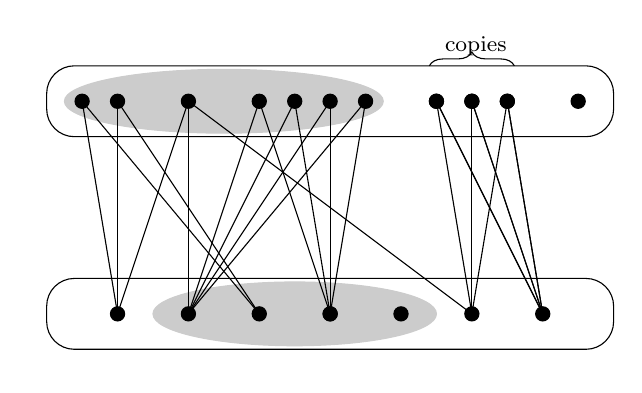
\begin{tikzpicture}[scale=.9]

\draw[rounded corners=10] (0,3) rectangle (8,4);
\draw[rounded corners=10] (0,0) rectangle (8,1);
\filldraw[black!20] (3.5, 0.5) ellipse (2 and 0.45);
\draw (3.5, 0.05) node[below] {};

\filldraw[black!20] (2.5, 3.5) ellipse (2.25 and 0.45);
\draw (2.5, 4) node[above=-2.5] {};


\draw (0,0.5) node[left] {};
\draw (0, 3.5) node[left] {};

\filldraw (4, .5) circle (0.1) node[below=2] {};

\foreach \x in {1,...,7}{
\filldraw (\x, .5) circle (0.1);
}


\foreach \x in {1,2,4,6,7,8,9,11,12,13,15}{
\filldraw (0.5*\x, 3.5) circle (0.1);
}
.

\draw [decorate,decoration={brace,amplitude=5pt}] (5.4, 4.0) --
node[above]{\footnotesize{ copies}} (6.6, 4.0);

\foreach \x in {1,...,3}{
\filldraw (5+0.5*\x, 3.5) circle (0.1) node[above=-1] {};

}


\foreach \x in {1,...,4}{
\draw (2.5+0.5*\x, 3.5)  -- (4,.5);

\draw (2.5+0.5*\x, 3.5)  -- (2,.5);

}

\draw (2, 3.5)  -- (2,.5);
\draw (1, 3.5)  -- (3,.5);

\draw (1, 3.5)  -- (1,.5);
\draw (.5, 3.5)  -- (1,.5);

\draw (.5, 3.5)  -- (3,.5);
\draw (2, 3.5)  -- (1,.5);


\draw (5.5, 3.5)  -- (6,.5);
\draw (6, 3.5)  -- (6,.5);
\draw (6.5, 3.5)  -- (6,.5);

\draw (2, 3.5)  -- (6,.5);


\draw (6.5, 3.5)  -- (7,.5);
\draw (6, 3.5)  -- (7,.5);
\draw (5.5, 3.5)  -- (7,.5);

\draw (6.5, 3.5)  -- (7,.5);
\draw (6, 3.5)  -- (7,.5);
\draw (5.5, 3.5)  -- (7,.5);

\end{tikzpicture}
\end{center}
\caption{\label{fig:bip}Graph  obtained from  by removing vertices from
 and duplicating each vertex  to its capacity. Shaded ellipses represent
sets used in Hall's theorem.}
\end{figure}

\begin{proof}
Consider a bipartite graph  with  if . Modify  to obtain  by removing vertices from 
and duplicating each vertex  to its capacity, i.e.\  times, see
also Fig.~\ref{fig:bip}.
Observe that cardinality- matchings in this graph correspond to
distance- solutions for . 
If any, such a matching can clearly be found in polynomial time.
We shall prove its existence by checking the deficit version of Hall's theorem,
i.e. that for each  we have 

First, observe that 
Moreover

Together these equalities conclude the proof.
\end{proof}

We proceed with a pair of simple properties of transfers. 
\begin{fact}\label{fct:comp}
Let  be a graph with  and a capacity function , and let .
Assume  is a distance- transfer of 
and  is a distance- transfer of . Then  is a
distance- transfer of .
\end{fact}
\begin{fact}\label{fct:image}
Let  and  be graphs with  and  and a
capacity function . Let  and let  be a monotonic function such that  for any
.
Assume  is a distance- transfer of . Then  is a
distance- transfer of .
\end{fact}

The following is the main technical contribution
of~\cite{svensson}.

\begin{lemma}[\cite{svensson}]\label{lem:tree}
Let  be a tree with a capacity function  and let  be a vector such that  for every non-leaf  and
.
Then one can find in polynomial time an integral 
distance-2 transfer of .
\end{lemma}

\subsection{Final rounding}
\label{ssec:tree-rounding}

\begin{lemma}
\label{lem:build-tree}
Let  be a connected bipartite graph
and let  such that  for every .
There exists an auxiliary tree  
such that  for any .
Moreover, such a tree can be computed in polynomial time.
\end{lemma}
\begin{proof}
We shall grow a tree adding a leaf in each step.
At the beginning we select any  and initialize with a single-vertex
tree.
Assume we have already grown a tree with vertex-set .
Choose a shortest path connecting  to . Such a path exists since
 is connected. If its length is at most 10, we add the endpoint in
 to the tree, joining it with the other endpoint.
For a proof by contradiction assume that a shortest path has length greater than
10. Since  is bipartite, its length needs to be even, and thus at least 12.
Choose the midpoint of such a path. Its distance both
to  and to  is at least 6, otherwise the path could be shortened.
This vertex contradicts the assumption that  for every .
\end{proof}

We are ready to prove Lemma~\ref{lem:tra}.

\begin{proof}[proof of Lemma~\ref{lem:tra}]
Since  is connected and every vertex of  is within distance  from~,
we can use Lemma~\ref{lem:build-tree} to construct a tree .
Let us add a duplicate  of every  to create a bipartite graph
, where  and .
For each  choose  and set  .
Let us create a tree  with .
We build it in two steps, see also Fig.~\ref{fig:tree}:
\begin{enumerate}
  \item create a tree with vertex set  so that  is an edge iff
  ,
  \item connect each vertex in  to the closest vertex
  in .
\end{enumerate}
Observe that endpoints of the edges created in the first step are at most at
distance 10 in , while endpoints of the edges created in the second step, at
most at distance 4.
Consequently,  for any .
Moreover, note that all non-leaves of  belong to .

\begin{figure}
\begin{center}
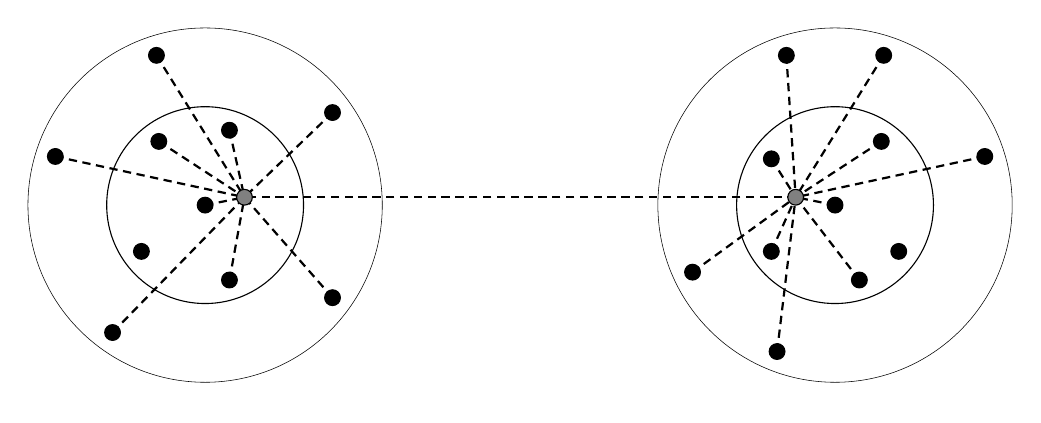
\begin{tikzpicture}[scale=1]
\draw[thick, densely dashed] (3.5, 0.1) -- (-3.5, 0.1);

\begin{scope}[xshift = 4cm, xscale=-1]
\filldraw (0,0) circle (0.1) node[right]{};



\filldraw (6*36:1) circle (0.1) node[above] {};

\foreach \x in {1,3.5,7,9}{
\filldraw (36*\x:1) circle (0.1);
\draw[thick, densely dashed] (36*\x:1) -- (.5,.1);
}

\foreach \x in {2,3,4.5,8.1, 9.3}{
\filldraw (36*\x:2) circle (0.1);
\draw[thick, densely dashed] (36*\x:2) -- (.5,.1);
}

\draw[thin] (0,0) circle (1.25);
\draw (0, -1.25) node[below=-2.5] {};
\draw[very thin] (0,0) circle (2.25);
\draw (0, -2.25) node[below=-2.5] {};

\draw[thick, densely dashed] (0, 0) -- (0.5, .1);
\draw[fill=gray] (0.5, 0.1) circle (0.1) node[left] {};

\end{scope}

\begin{scope}[xshift = -4cm]

\filldraw (0,0) circle (0.1) node[left]{};


\filldraw (6*36:1) circle (0.1) node[above] {};

\foreach \x in {2,3.5,8}{
\filldraw (36*\x:1) circle (0.1);
\draw[thick, densely dashed] (36*\x:1) -- (.5,.1);
}

\foreach \x in {1,4.5, 6.5,3,9}{
\filldraw (36*\x:2) circle (0.1);
\draw[thick, densely dashed] (36*\x:2) -- (.5,.1);
}

\draw[thin] (0,0) circle (1.25);
\draw (0, -1.25) node[below=-2.5] {};
\draw[very thin] (0,0) circle (2.25);
\draw (0, -2.25) node[below=-2.5] {};
\draw[thick, densely dashed] (0, 0) -- (0.5, .1);
\draw[fill=gray] (0.5, 0.1) circle (0.1) node[right] {};
\end{scope}
\end{tikzpicture}
\end{center}
\caption{\label{fig:tree}
A fragment of the tree  with . Nodes of  are
marked in black, of  in gray. Edges of  are represented as dashed lines.
Note that  and  are not vertices of .}\
\end{figure}
 Let  be a feasible solution of . Note that 
can be interpreted as a vector in  extending with zeroes at .
We shall give an integral distance-24 transfer  of .
Despite it being formally a transfer in ,  will be a subset of , i.e. a
transfer of   as well.

Recall that by (\ref{it:two}), the sets
 are pairwise disjoint and in particular  are pairwise different. 
This lets us use~\eqref{eq:near} to gather in  one unit from  for
every  so that the whole value in 
is transferred to .
Note that  for each , so
this way we obtain a distance-2 transfer  of . Additionally, we
have made sure that , so  can be interpreted as a vector in
, and that , so  is 1 for all non-leaves of
. This lets us use Lemma~\ref{lem:tree} to obtain an integral distance-2 transfer  of . According to
Fact~\ref{fct:image} it can be interpreted as a distance-20 transfer of
. Finally we move the value from  to  for each .
Note that these vertices have equal capacities, so this step can be interpreted
as an integral distance-2 transfer.

The final transfer is therefore a composition
of a distance-2 transfer, a distance-20 transfer and a distance-2 transfer.
Thus, by Fact~\ref{fct:comp} it is a distance-24 transfer.\footnote{A simpler
construction gives a distance- transfer, without introducing additional
vertices . It is enough first to gather one unit from  in  and build 
a tree on vertices , where adjacent vertices of the tree are at distance
at most  in . By using Lemma~\ref{lem:tree} one obtains a distance-28 transfer,
which together with the initial distance-2 transfer gives an integral distance-30 transfer.}
By Lemma~\ref{lem:app} having an integral distance-24 transfer
is enough to construct a distance-25 solution  in polynomial time,
which concludes the proof of Lemma~\ref{lem:tra}.
\end{proof}

\section{Wrap-up}
\label{sec:wrap-up}

With the results of previous section, we are ready to the prove the
main theorem.
\begin{theorem}\label{thm:gen}
The \fullsup\  problem admits a 25-approximation algorithm.
\end{theorem}
\begin{proof}
Section~\ref{sec:thresholding} with Algorithm~\ref{alg:red} provides (a Turing-like)
reduction to graphic instances. 
Algorithm~\ref{alg:pre} of Section~\ref{sec:skeleton} given such an instance outputs several sets. 
Provided that a distance-1 solution exists, one of them is guaranteed to
be a skeleton. Each of these sets is then processed separately. As described
in Section~\ref{sec:clustering}, some redundant vertices are removed and the graph is
partitioned into connected components. Dynamic programming (Lemma~\ref{lem:dp})
is then used to find a compatible partition of  and , 
so that each linear program  admits a feasible solution.
While this procedure might fail in general, it is guaranteed to succeed for a skeleton, hence at least once if a distance-1 solution exists. 


Note that if such a partition is found, then for each
of the instances  together with sets ,
we can use Lemma~\ref{lem:tra} as all the conditions  are satisfied.
A sum of solutions for these  instances is finally
returned as a distance-25 solution for the original graphic instance.
\end{proof}

\section*{Acknowledgements}

We would like to thank Samir Khuller for suggesting the study of this variant
of the -{\sc center} problem and helpful discussions.



\bibliography{kcenter}

\newpage
\appendix

\section{Soft capacities and uniform capacities}\label{sec:improvements}
\label{app:improvements}
\subsection{Soft capacities}
A variant of \fullsup\ with soft capacities can be easily reduced to the
original problem preserving the quality of solutions.
It suffices to duplicate  times each .
Opening several facilities in  then corresponds to opening facilities in
several copies of .
\begin{theorem}
The \fullsup\  problem with soft capacities admits a 25-approximation algorithm.
\end{theorem}

\subsection{Uniform capacities}
In the special case of \fullsup\  where the capacities are uniform,
we can obtain a slightly better approximation factor.
Namely, in the proof of Lemma~\ref{lem:tra} 
we can set  and avoid introducing additional vertices , using  instead. With this change the
third component of the transfer -- moving the value from  to  -- is not
necessary, thus we get an integral distance-22 transfer. Analogously to
Theorem~\ref{thm:gen}, we then obtain the following result.
\begin{theorem}
The \fullsup\  problem with uniform capacities admits a 23-approximation algorithm.
\end{theorem}

\subsection{Uniform soft capacities}
While we could argue as for general soft capacities that in the case of uniform
soft capacities we have a 23-approximation algorithm, a tailor-made proof gives
much better factor.

It is easy to verify that the ingredients of the proof of
Theorem~\ref{thm:gen} be adapted to soft capacities with two changes:
\begin{itemize}
  \item instead of a set of open facilities, we consider a multiset,
  \item we drop the  requirement in the LP.
\end{itemize}
Thus, in order to obtain an -approximation algorithm it is enough to compute an integral (again, multisets
allowed) distance- transfer of , where  is the fractional solution
of the LP for an instance satisfying the conditions of Lemma~\ref{lem:tra}.

Again, we shall start with gathering value from  in . This time we
are allowed to gather more than one unit in , so we gather everything from
. A vector  defined this way clearly is a distance-2
transfer of . Moreover, by~\eqref{eq:near} at least one unit is gathered
at each . Like in the proof of Lemma~\ref{lem:tra}, the second component
relies on the structure of .
We connect each  to the closest  obtaining a tree .
This way we have a tree on  whose non-leaves belong to , and
such that  for any .
We shall give an integral distance-1 transfer  of .
Let us make  a rooted tree, setting the root at a vertex .
For each  define  as the sum of  over all descendants  in the
subtree rooted at . 
For each  we transfer  units from  to
its parent .  Note that  is an integer, since , so  and the operation is well defined. 
Observe that for every  it holds that

 Also, for any vertex  we have . That is because for leaves
 and for the remaining vertices , since  so that .
Consequently, for any , setting , we get

since  for any . Moreover  is a constant, so this inequality 
proves the condition \ref{it:nei}. of Definition~\ref{def:tra}, and thus  is indeed a distance-1 transfer of .
By Fact~\ref{fct:image} this defines a distance-10 transfer of ,
which composed with the previous transfer using Fact~\ref{fct:comp} gives an
integral distance-12 transfer of .
Consequently, repeating the proof of Theorem~\ref{thm:gen} we get the
following result.
\begin{theorem}
The \fullsup\  problem with uniform soft capacities admits a 13-approximation
algorithm.
\end{theorem}


\section{Equivalence of \textsc{Capacitated} -\textsc{supplier with Outliers} and \textsc{Capacitated} -\textsc{center with Outliers}}\label{app:equivalence}

\begin{theorem}
Assume there exists an -approximation algorithm for \textsc{Capacitated} -\textsc{center with Outliers}.
Then there exists an -approximation algorithm for \textsc{Capacitated} -\textsc{supplier with Outliers}.
\end{theorem}
\begin{proof}
Let us consider an instance  of \textsc{Capacitated} -\textsc{supplier with Outliers}.
Define an instance  of \textsc{Capacitated} -\textsc{center with Outliers} as
follows: take  where , and
for every  set . Other values of  
are taken as the symmetric, transitive closure of those determined explicitly (note that since  was symmetric and satisfied triangle equality,
the closure does not modify any explicitly set value of ).
Also, set  for ,  for , , and .
Clearly  can be constructed in polynomial time from .
Thus, it suffices to show that a distance- solution exists in  if
and only if a distance -solution exists in .

One direction is very simple: assume  is a distance- solution in .
Observe that  defined as 
for  is a distance- solution in .

Now, let us prove the other implication. The construction is going
to be similar to the one in the proof of Lemma~\ref{lem:app}.
Assume  is a distance-
solution in . Note that  may contain vertices from .
Construct a bipartite graph  with  if ,
and modify  to obtain  by removing vertices from  and multiplicating each 
to its capacity, i.e.\  times.
Note that , so  a cardinality- matching in  gives a distance- solution to .
Observe that for any  and , it holds that .
Consequently, for any 
 we have the following inequality

Therefore

Both sides of this inequality are integral, which implies 

and, by the deficit version of Hall's theorem, also guarantees the existence of a cardinality -matching in  and a distance -solution to .
\end{proof}

\section{Connected instance with arbitrarily large integrality gap}\label{app:example}
\begin{fact}
For arbitrarily large  there is a graphic instance  of \fullsup\ 
and a set , such that all conditions of Lemma~\ref{lem:tra} except (\ref{it:three}) are satisfied,
but  does not have a distance- solution.
\end{fact}
\begin{proof}
Assume  and fix .
Let  consist of the following components (see also Figure~\ref{fig:ex}): a path of  vertices with endpoints  and inner vertices alternately in  and , four vertices  (), with  adjacent to ,
and  vertices  (), with  adjacent both to  and .
For each  we set , moreover  and . The set  is defined as .

\begin{figure}
\begin{center}

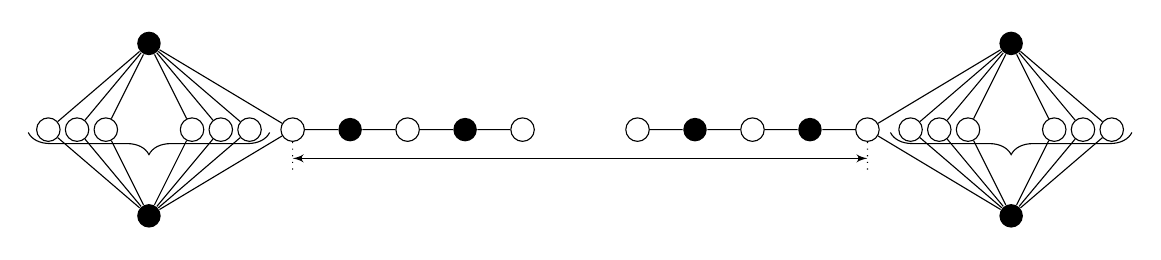
\begin{tikzpicture}[scale=.73,every node/.style={circle, inner sep = 3, }]
\foreach \x in {1,2} {
 \foreach \y in {1,2} {
	\node[fill=black,circle] (f\x\y) at (\x*15,\y*3) {};
}
    \draw (\x*15,3)  node[below=-3] {\footnotesize{}};
    \draw (\x*15,6)  node[above=-3] {\footnotesize{}};


}
\foreach \x in {1,2} {
\draw[decorate, decoration={brace, amplitude=8}] (\x*15+2.1,4.45) -- node[below=2]{\footnotesize{}} ( \x*15-2.1,4.45);
\draw (\x*15, 4.5) node {};
\foreach \y in {0,1,2} {
		\node[draw=black,circle] (c\x\y) at (\x*15-0.75-\y/2,4.5) {};
		\draw (f\x1) -- (c\x\y) -- (f\x2);
}
\foreach \y in {0,1,2} {
		\node[draw=black,circle] (d\x\y) at (\x*15+0.75+\y/2,4.5) {};
		\draw (f\x1) -- (d\x\y) -- (f\x2);
}
}
\foreach \x in {1,2} {
\node[draw=black,circle] (c\x) at (7.5+\x*10, 4.5) {};
\draw (7.5  + \x*10, 4.5) node[left=-9.5] {\footnotesize{}};
\draw (f\x1) -- (c\x) -- (f\x2);
}

\foreach \x in {0,2,6,8} {
 \node[fill=black,circle] (a\x) at (18.5+\x, 4.5) {};	
}
\foreach \x in {1,3,5,7} {
 \node[draw=black,circle] (a\x) at (18.5+\x, 4.5) {};	
}
\draw (c1) -- (a0) -- (a1) -- (a2) -- (a3) ;
\draw (c2) -- (a8) -- (a7) -- (a6) -- (a5) ;
\draw (22.5,4.5) node {};

\draw[dotted] (c1) -- (17.5,3.8)  (c2) -- (27.5,3.8);
\draw[arrows={latex'-latex'}] (17.5, 4) -- node[below] {\footnotesize{}} (27.5, 4);

\end{tikzpicture}
\end{center}
\caption{\label{fig:ex}
The graph , vertices in  are marked as white circles, vertices in  as black circles.}

\end{figure}
 Observe that an instance  constructed this way satisfied conditions of Lemma~\ref{lem:tra} except (\ref{it:three}):
clearly  is connected, . Consider a solution  of  with the following
non-zero coordinates:  for ,  for , .
It is easy to verify that it is a feasible solution.

It remains to show that  does not have a distance- solution.
For a proof by contradiction, assume that is does, with  being the set of open facilities and 
being the set of clients served.
Note that each  must serve  clients, since  and  for .
Let  and  for .
Observe that  and the sum is disjoint. Consequently  and   for some .
However,  does not contain  for any , so , a contradiction.
\end{proof}




\end{document}
